\clearpage
\appendices

\section{Khảo sát cấu hình và đặc điểm giao dịch}
\label{app:fashion_configuration}

\textit{Kích thước vùng ảnh.}
Lưới không chồng lấn trên ảnh $28\times28$ tạo 196, 49 hoặc 16 vùng khi cạnh vùng lần lượt là 2, 4 hoặc 7 pixel. Vùng nhỏ cho phép lọc nền chi tiết hơn nhưng làm tăng số vectơ cần xử lý. Vùng lớn chứa nhiều điểm ảnh lân cận hơn và có thể trộn nền với các đường biên của vật thể. Trong phép đối chiếu $4\times4$ với $7\times7$, ở mức loại khoảng 39,3\% số vùng, tỷ lệ gradient bị mất lần lượt là 5,92\% và 14,00\%. Lưới cố định cũng khiến mẫu điểm ảnh phụ thuộc vào vị trí của đường biên so với lưới.

\textit{Lọc nền.}
Bảng~\ref{tab:fashion_filter_appendix} so sánh các cấu hình trong khảo sát ảnh. Tỷ lệ mất gradient được tính bằng tổng độ lớn gradient trong các vùng bị loại chia cho tổng độ lớn gradient trên ảnh gốc. Với ngưỡng 29, mỗi ảnh còn trung bình 30,62 vùng và mọi ảnh đều còn ít nhất một vùng.

\begin{center}
    \captionof{table}{Ảnh hưởng của ngưỡng lọc trên lưới $4\times4$}
    \label{tab:fashion_filter_appendix}
    \footnotesize
    \begin{tabular}{@{}lrrr@{}}
        \toprule
        Cấu hình & Vùng loại & Mất gradient & Mất hết vùng \\
        \midrule
        Giữ mọi vùng      & 0,00\%  & 0,00\% & 0 \\
        Ngưỡng 29 (Q10+) & 37,50\% & 4,41\% & 0 \\
        Ngưỡng 97 (Otsu) & 43,30\% & 8,90\% & 0 \\
        \bottomrule
    \end{tabular}
\end{center}

\textit{Đặc trưng và số cụm.}
Vectơ gồm 16 mức xám theo thứ tự cột, vì vậy bình phương khoảng cách Euclid cộng chênh lệch bình phương tại các vị trí tương ứng. Biểu diễn này giữ bố cục điểm ảnh trong vùng nhỏ và nhạy với thay đổi độ sáng, dịch chuyển hoặc xoay. Bảng~\ref{tab:fashion_k_appendix} ghi kết quả khảo sát ở cùng giá trị khởi tạo ngẫu nhiên 123. Khi số cụm tăng, các lượt khảo sát cho độ méo thấp hơn và giao dịch dài hơn.

\begin{center}
    \captionof{table}{Đánh đổi giữa độ méo và độ dài giao dịch}
    \label{tab:fashion_k_appendix}
    \footnotesize
    \begin{tabular}{@{}rrrr@{}}
        \toprule
        $K$ & Độ méo & Số mã TB & Hội tụ \\
        \midrule
        16  & 0,441 &  9,00 & Có \\
        32  & 0,347 & 12,27 & Có \\
        64  & 0,271 & 15,11 & Có \\
        128 & 0,219 & 17,99 & Có \\
        256 & 0,177 & 20,29 & Chưa \\
        \bottomrule
    \end{tabular}
\end{center}

\textit{Giao dịch dùng trong báo cáo.}
Sau khi bỏ các mã lặp trong từng ảnh, 70.000 giao dịch có tổng cộng 859.100 lượt xuất hiện của 32 mã phân biệt. Độ dài giao dịch từ 2 đến 26, với trung vị 12 và độ lệch chuẩn 3,06 mã. Mật độ, tính bằng $859\,100/(70\,000\times32)$, là 38,35\%.
Thống kê trên được tính trực tiếp từ bộ giao dịch dùng trong báo cáo.
Xem \href{https://github.com/NguyenVoTanDuy2006/DataMining-FIM-Project/blob/e8390ba36d55e79c3ea8258d4d56de6385a8b733/docs/UD2/TC_plan.md}{khảo sát tiền xử lý ảnh} và \href{https://github.com/NguyenVoTanDuy2006/DataMining-FIM-Project/blob/e8390ba36d55e79c3ea8258d4d56de6385a8b733/notebook/UD2/experiments/EDA2_FashionMNIST_Transaction_Evaluation.ipynb}{khảo sát giao dịch}.

\newpage
\section{Đối chiếu Eclat và cách đọc số đo}
\label{app:fashion_eclat}

\textit{Độ hỗ trợ trên BoVW nhị phân.}
Gọi $D(w)$ là tập giao dịch chứa từ thị giác $w$ và $N$ là số giao dịch. Độ hỗ trợ của tập mục $X$ là
\[
    \operatorname{supp}(X)
    = \frac{\left|\bigcap_{w\in X} D(w)\right|}{N}.
\]
Ví dụ minh họa, với ba giao dịch $\{1,6\}$, $\{6,24\}$ và $\{1,6,24\}$, cặp $\{1,6\}$ xuất hiện ở giao dịch thứ nhất và thứ ba nên có độ hỗ trợ $2/3$. Histogram tần suất giữ được số lần lặp và cần thêm quy tắc mã hóa nếu dùng với Eclat. BoVW theo vùng giữ vị trí gần đúng bằng cách gắn mã với từng vùng. Cách này làm tăng số mục và có thể chia lượt xuất hiện của một mã giữa nhiều mục.

\textit{Đối chiếu kết quả.}
Nhóm chạy hai \href{https://github.com/NguyenVoTanDuy2006/DataMining-FIM-Project/tree/e8390ba36d55e79c3ea8258d4d56de6385a8b733/src/algorithm}{bản cài đặt Eclat} trên cùng một bộ giao dịch. Ở cả sáu ngưỡng, hai bản trả về cùng các tập mục và cùng số ảnh chứa từng tập. Cột \emph{Sai hỗ trợ} trong Bảng~\ref{tab:fashion_audit_appendix} ghi số tập mục có độ hỗ trợ tính lại khác với kết quả đã trả về.

\begin{center}
    \captionof{table}{Đối chiếu độ hỗ trợ và RSS theo ngưỡng}
    \label{tab:fashion_audit_appendix}
    \footnotesize
    \setlength{\tabcolsep}{3.5pt}
    \begin{tabular}{@{}rrrrr@{}}
        \toprule
        Ngưỡng & Số tập & Sai hỗ trợ & Set (MiB) & BitVector (MiB) \\
        \midrule
        80\% &     0 & 0 & 436,14 & 445,52 \\
        60\% &     2 & 0 & 440,89 & 436,34 \\
        40\% &    15 & 0 & 462,65 & 432,62 \\
        20\% &   174 & 0 & 477,53 & 433,88 \\
        10\% & 1.275 & 0 & 521,41 & 447,99 \\
         5\% & 7.228 & 0 & 540,73 & 443,43 \\
        \bottomrule
    \end{tabular}
\end{center}

\textit{Diễn giải thời gian và bộ nhớ.}
Khi thêm một mục, số giao dịch chứa tập mới chỉ có thể giữ nguyên hoặc giảm. Hạ ngưỡng giúp nhiều nhánh vượt qua bước cắt tỉa, nên Eclat có thể phải xét thêm các phép giao. Bản Set giao các tập số nguyên. Bản BitVector đếm trước các mục đơn để chỉ cấp phát vectơ bit cho những mục đạt ngưỡng, rồi dùng phép AND và đếm bit bật. Chi phí giao có thể góp phần vào chênh lệch quan sát được ở ngưỡng 5\%.

Mỗi cấu hình được đo một lượt trong một tiến trình riêng, chạy Julia 1.13.3 trên Linux với một luồng và giới hạn 3.072 MiB. Tổng thời gian bao gồm khởi tạo, nạp dữ liệu, khai thác và ghi kết quả. RSS đo lượng bộ nhớ vật lý cực đại của cả tiến trình. Để biết mức chênh lệch có ổn định hay không, cần đo lặp từng cấu hình. Xem \href{https://github.com/NguyenVoTanDuy2006/DataMining-FIM-Project/blob/e8390ba36d55e79c3ea8258d4d56de6385a8b733/notebook/UD2/release/03_frequent_itemset_mining.ipynb}{notebook thực nghiệm Eclat}.

\onecolumn
\section{Hình minh họa bổ sung cho các mẫu đại diện}
\label{app:fashion_patterns}

Ba hình dưới đây bổ sung cho Hình~\ref{fig:visual_pattern_4_12_24} trong thân bài. Mỗi hình đặt tâm cụm và vùng ảnh thật cạnh các ảnh chứa mẫu. Ảnh ngoài cùng bên phải thiếu ít nhất một mã của mẫu.

\begin{center}
    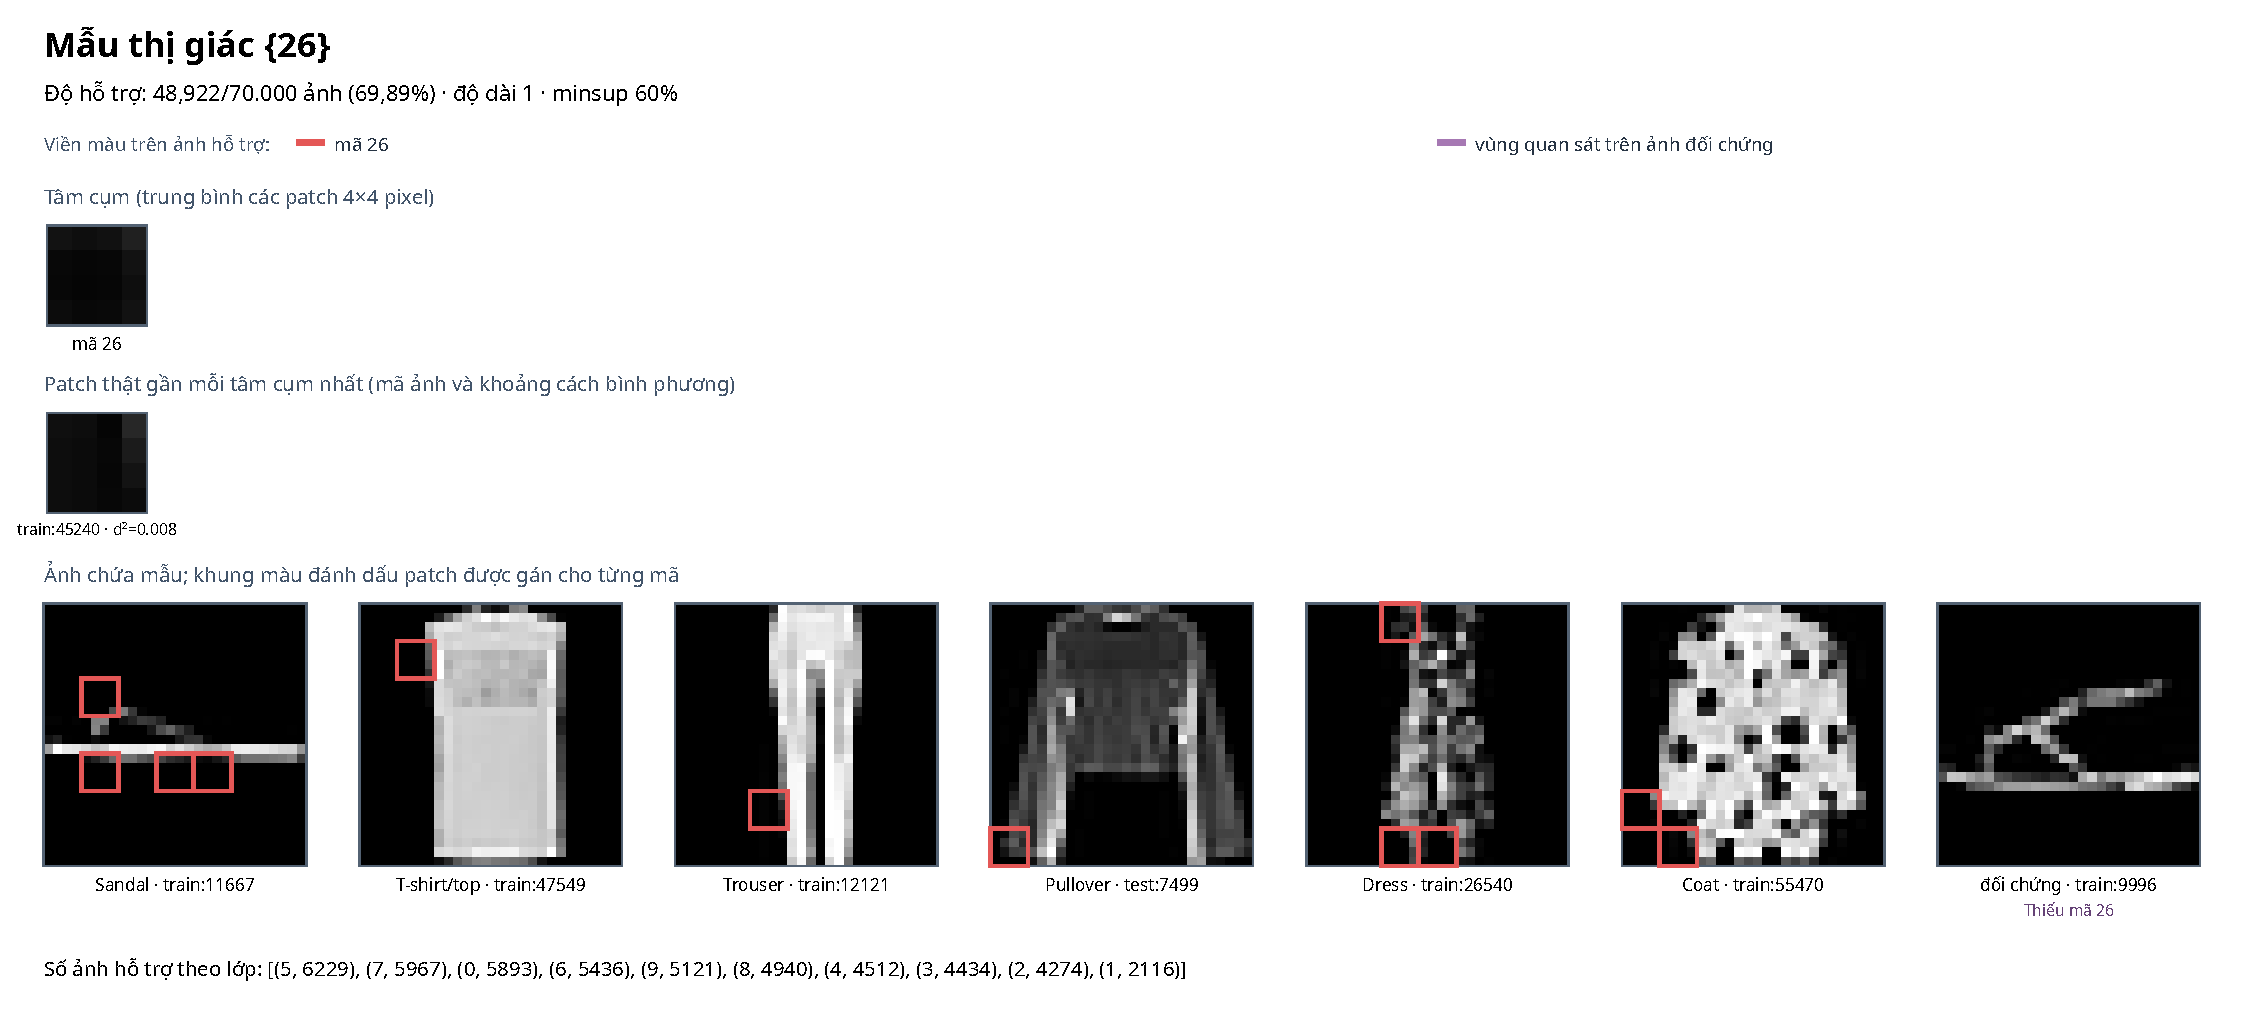
\includegraphics[width=0.97\textwidth,height=0.25\textheight,keepaspectratio]{figures/appendix/pattern_26.pdf}
    \captionof{figure}{Mẫu $\{26\}$. Tâm cụm chủ yếu có mức xám thấp. Các vùng gán mã 26 xuất hiện ở nhiều vị trí, chẳng hạn gần quai dép hoặc mép áo trong các ảnh minh họa.}
    \label{fig:fashion_appendix_26}
\end{center}

\begin{center}
    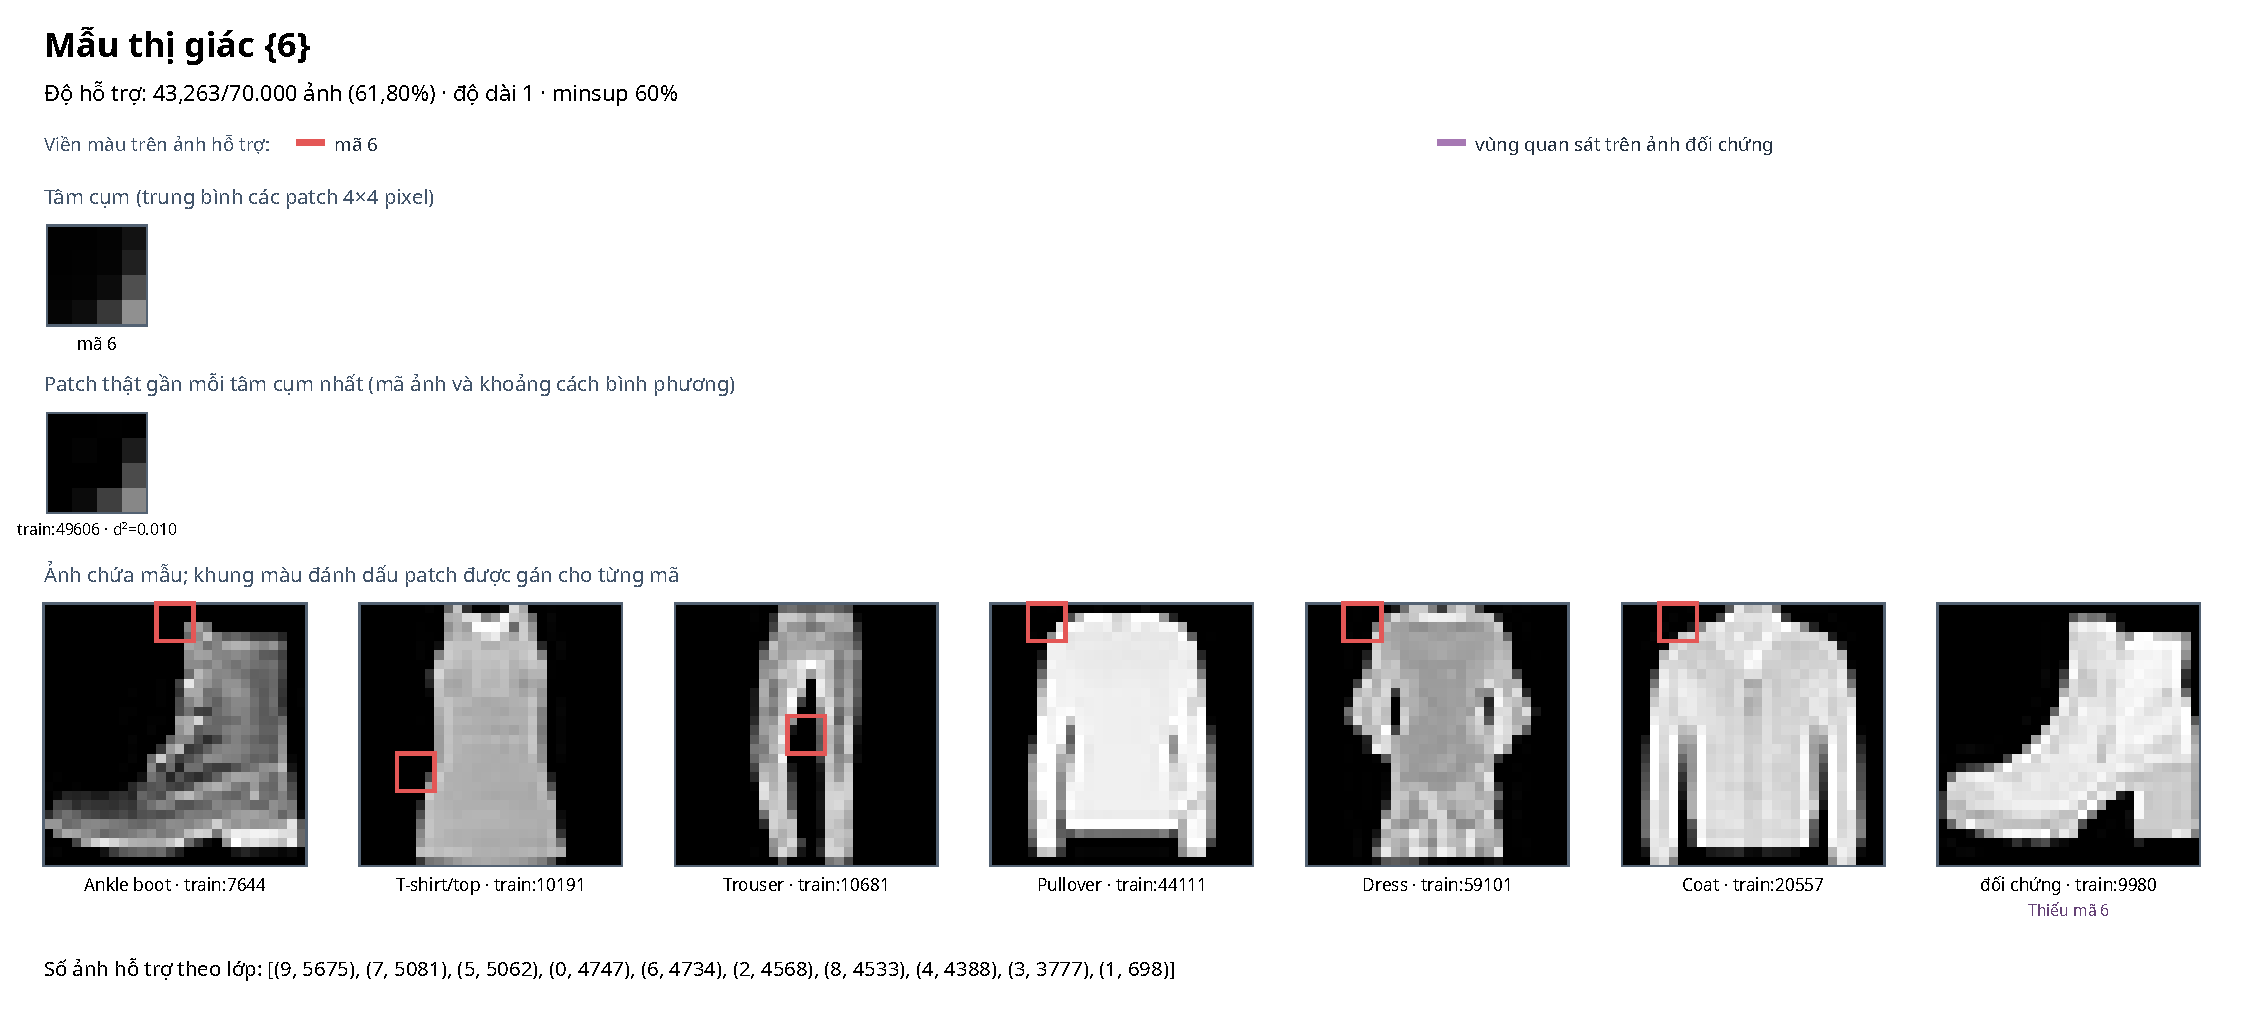
\includegraphics[width=0.97\textwidth,height=0.25\textheight,keepaspectratio]{figures/appendix/pattern_6.pdf}
    \captionof{figure}{Mẫu $\{6\}$. Tâm cụm chuyển từ vùng tối sang vùng sáng hơn ở một góc. Các vùng được đánh dấu cho thấy dạng chuyển mức xám này xuất hiện trên nhiều loại trang phục.}
    \label{fig:fashion_appendix_6}
\end{center}

\begin{center}
    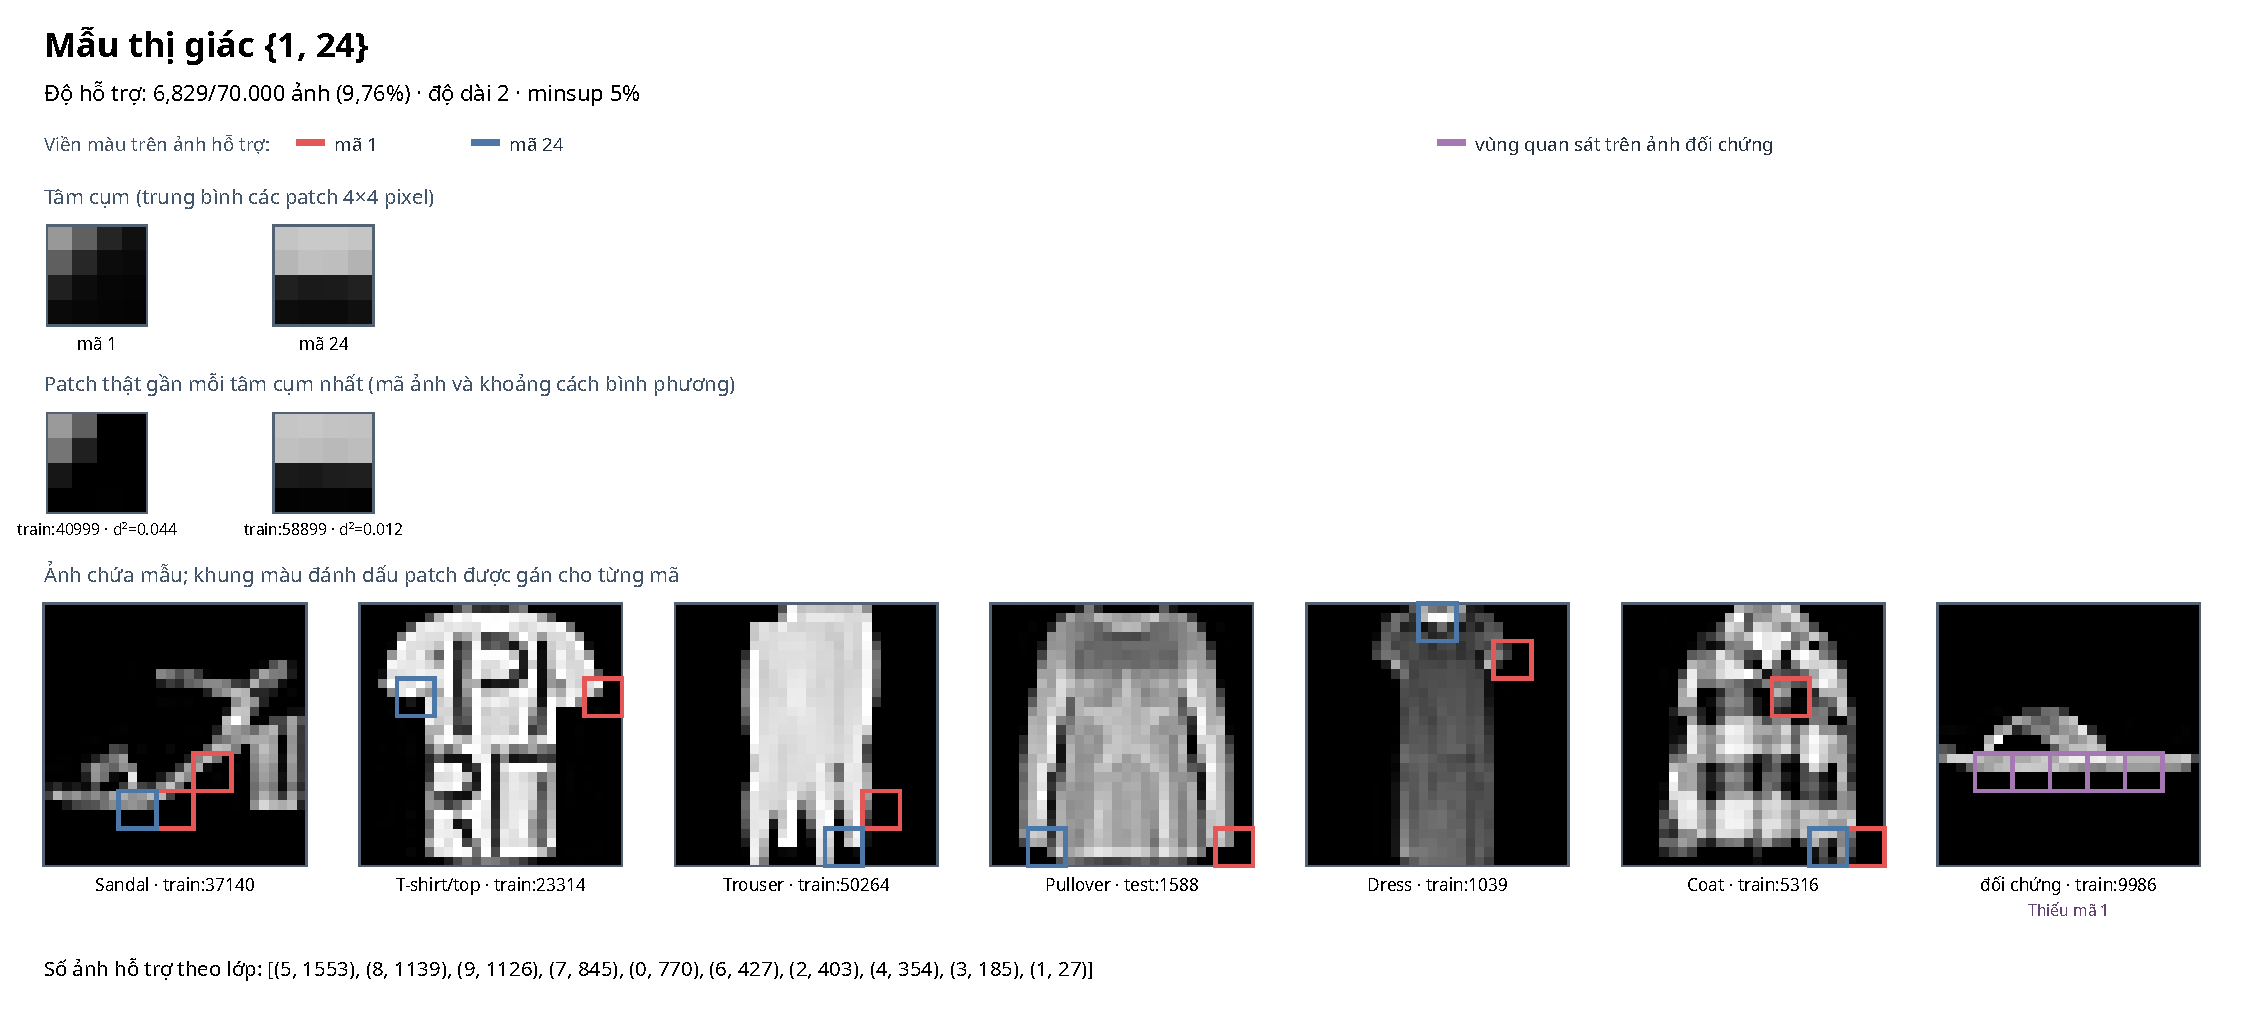
\includegraphics[width=0.97\textwidth,height=0.25\textheight,keepaspectratio]{figures/appendix/pattern_1_24.pdf}
    \captionof{figure}{Mẫu $\{1,24\}$. Mã 1 thể hiện chuyển sáng tối theo đường chéo, còn mã 24 có dải tối ở phần dưới. Các vùng mang hai mã có thể nằm ở những vị trí khác nhau trong cùng ảnh.}
    \label{fig:fashion_appendix_1_24}
\end{center}
